%!TEX root = ../thesis.tex

\chapter{Implementation}
\label{cha:implementation}
In this chapter, I describe the design and implementation of the developed web front end. First, I introduce the application's high-level architectural components, explain the interactions between them and give an overview of their deployment specifics. Then, I list the different word embedding and domain-specific data sets used in the web application's database. Most importantly, I describe the implementation of the web application's front and back end, including the reasons for choosing the specific technologies used.

The web application's source code was licensed under the terms of the free software MIT license and can be found in a GitLab repository\footnote{\url{https://gitlab.com/yanakiev/freddyDemo}}.

\section{Architectural Overview}
\label{sec:architecture}
\subsection{High-Level Design}
\begin{figure}
	\centering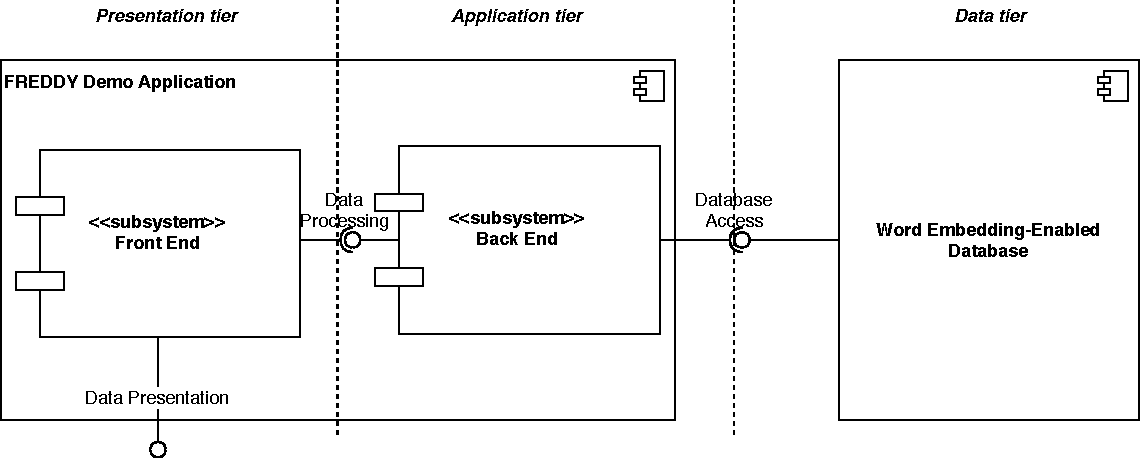
\includegraphics[width=\textwidth,keepaspectratio]{impl_architecture_component.pdf}
	\caption{A component diagram showing the web application's three-tier architecture.}
	\label{fig:architecture_component}
\end{figure}
The software solution's architecture is based on a classic \textit{three-tier} web application architecture. A three-tier architecture is a \textit{client-server} software architecture pattern. It separates the user interface of the application (the \textit{presentation tier}), the functional logic (the \textit{application tier}) and the data storage and access (the \textit{data tier}). Not only does it provide the advantages of modularity, speed of development, scalability and performance, but it also allows the independent replacement of any of its components. For example, one can use any user interface without modifying the data processing component behind it. Furthermore, many well-established modern web development stacks are based on this model. These advantages make the three-tier architecture especially well-suited to the demo application's use cases. Figure \ref{fig:architecture_component} shows the different components that constitute the application's architecture. A detailed description of technologies and languages used in the application's components follows in the next sections.

The data tier comprises both the data sets used in the web application and the database management software that manages and provides access to the data. It consists of the word-embedding-enabled relational database system and is the data source for the web application. It provides access to word embedding operations and stored data sets to the next tier in the architecture, the application tier.

The application tier, also called \textit{back end}, provides a middleware between the data tier and the presentation tier and drives the application's core capabilities. It extracts information from the database at the front end's request, processes it, dynamically generates data based on it and forwards it to the presentation tier. The back end can also relay other types of commands to the database, such as adjusting the database's settings. It also provides the functionalities of a classic web server, serving the web application's static content.

The web application's user directly accesses the presentation tier, also called \textit{front end}. The user can achieve the different use cases by interacting with its graphical user interface. The front end of the web application requests dynamic and static data from the back end and displays content and information useful to the end user, such as the results of a word embedding SQL query.

\subsection{Deployment Model}
\begin{figure}
	\centering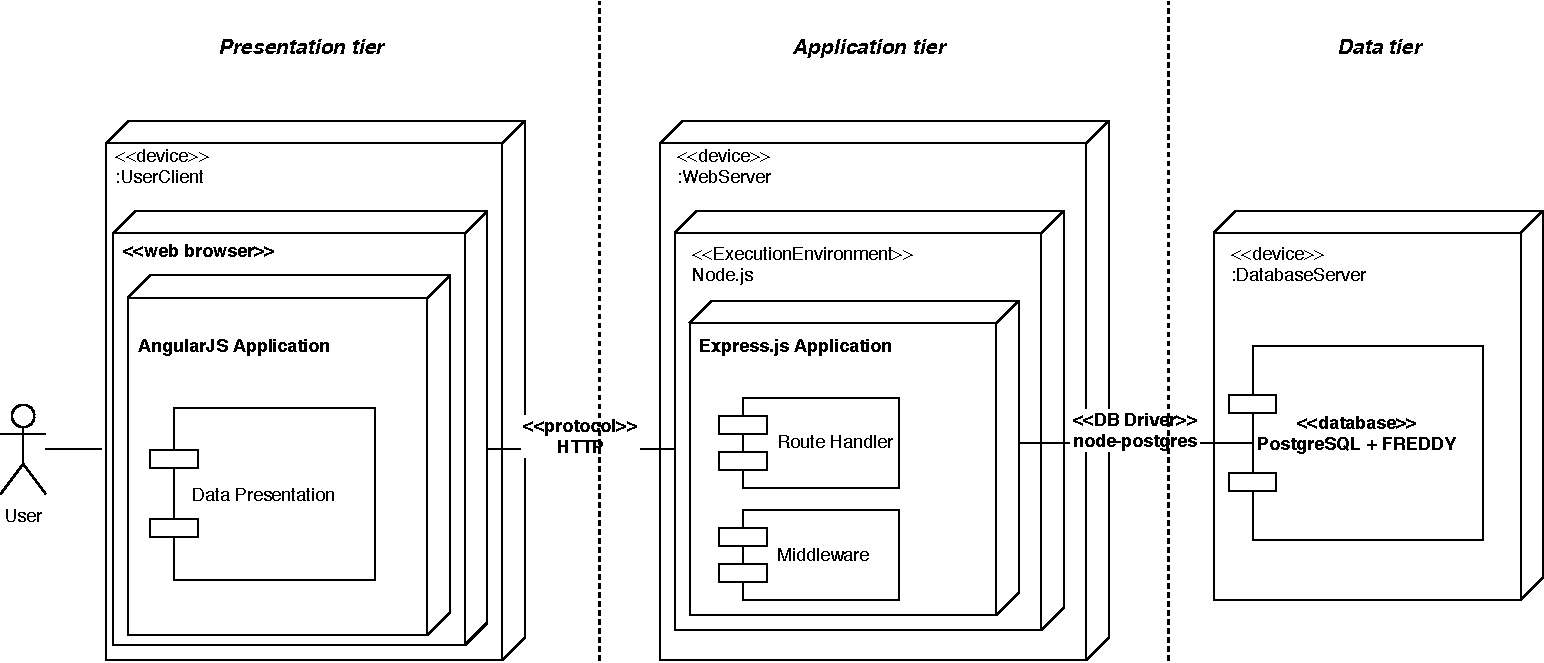
\includegraphics[width=\textwidth]{impl_architecture_deployment.pdf}
	\caption{A diagram detailing the web application's deployment.}
	\label{fig:architecture_deployment}
\end{figure}
Figure \ref{fig:architecture_deployment} shows the demo application's distributed deployment model\footnote{The web application's components may also run on the same physical machine.}. The user accesses the web application's front end using a conventional web browser running on their own device. The front end was realized as an \textit{AngularJS} application and provides a way for the user to retrieve query results, examine them, adjust word embedding settings and measure the database's performance using graphical interaction paradigms. In other words, it is responsible for the presentation of data obtained from the back end in a user-friendly manner. The front end and the back end, which runs on a web server device, communicate over HTTP using asynchronous RESTful API calls. The back end was implemented as an \textit{Express.js} application written in JavaScript and running in the \textit{Node.js} run-time environment. It consists of a route handler which redirects requests from the front end to the relevant API functions and other middleware. The middleware itself has facilities for both handling a conventional web server's tasks and API functions specially implemented for accessing FREDDY's capabilities. The back end communicates with the database using a PostgreSQL driver for Node.js. The database system, consisting of a PostgreSQL system with word embeddings data sets and installed FREDDY extensions, runs on another device called a database server.

\section{Database}
The relational database management system powering the web application is a standard PostgreSQL 10.4 installation running on an Ubuntu 16.04 virtual machine. In addition, the word embedding extensions provided by FREDDY have been installed into the database system, giving access to all word embedding operations implemented by it. Several word embeddings and domain-specific data sets have also been imported into the database in order to use word embedding queries in the demo application.

The web application provides examples of ten predefined queries using word embeddings on the domain-specific data sets. The predefined queries are stored in a JSON file using a custom format on the web application's back end. Adding new predefined queries is as simple as appending a new entry to the JSON file (see Table \ref{tab:queries_json} in Appendix \ref{sec:queries_format} for its technical description). 

\subsection{Word Embeddings Data Sets}
\label{sec:datasets}
The database contains three different pre-trained sets of word embeddings, each of them including the index tables required by FREDDY's high-performance word embedding operations.

The first set of word embeddings was trained on part of the data set of \textit{Google News} using the word2vec algorithm and contains 300-dimensional vectors for 3 million words and phrases. Considering the broad range of topics covered in the Google News corpus, this data set is suitable for extracting semantic information in different areas, such as entertainment, current events or science. Its downside is that it was trained on news from only the last ca. 10 years, and thus covers only recent events and topics. The second word embeddings data set was trained on data from \textit{Wikipedia}, and the last one contains vector representations trained using the \textit{GloVe}\footnote{\url{https://nlp.stanford.edu/projects/glove/}} unsupervised learning algorithm. The index structures for the three word embeddings data sets were created using the tools bundled with FREDDY.

\subsection{Domain-Specific Data Sets}
Three domain-specific data sets from various areas of human knowledge were imported into the database in order to give different users an idea about the capabilities of word embeddings and their uses in relational databases.

\textit{IMDb\footnote{\url{https://www.imdb.com/}}} is an online database of information about films and television programs, including cast, production crew and personnel biographies and plot summaries. It contains more than 250 million data items including more than 4 million movies or other programs and 8 million cast and crew members \cite{imdb-about}. As movies and TV are an integral part of pop culture, this data set was chosen to demonstrate FREDDY's capabilities in a way that is easily understandable for almost everyone. The IMDb data set was imported using the \textit{imdbpy2sql\footnote{\url{https://github.com/alberanid/imdbpy}}} command-line tool by Davide Alberani.

\textit{Discogs\footnote{\url{https://www.discogs.com}}} is a crowdsourced database of information about audio recordings, including commercial releases, promotional releases, and bootleg or off-label releases. More than 415,000 people have contributed their knowledge to it, to build up a catalog of more than 9,900,000 recordings and 5,700,000 artists \cite{discogs-about}. Users of the web application can extract semantic information about their favorite bands or artists and their body of work by querying the Discogs database. The Discogs data set was imported using the \textit{discogs2pg\footnote{\url{https://github.com/alvare/discogs2pg}}} tool written by Ezequiel A. Alvarez.

The last data set used in the demo application's setup is \textit{dblp\footnote{\url{https://dblp.uni-trier.de/}}}. It is the online reference for bibliographic information on major computer science publications and indexes over 3.3 million publications, published by more than 1.7 million authors. To this end, dblp indexes about than 32,000 journal volumes, more than 31,000 conference or workshop proceedings, and more than 23,000 monographs \cite{dblp-about}. By querying the dblp data set, the user can extract information about the relationships between the authors of publications and other semantic data.

\section{Back End}
The web application's back end was developed using the \textit{Node.js} web framework \textit{Express.js} and was written in ECMAScript 6-compatible JavaScript. Node.js is a server-side runtime environment	that lets developers use JavaScript for server-side scripting. It has an event-driven architecture capable of asynchronous I/O. Furthermore, it has the largest ecosystem of open source libraries in the world, which include database drivers and components for front and back end development. This facilitates the task of quick development of web applications by providing ready solutions to frequently encountered problems in web development. Express.js is a web application framework which functions as a thin layer of fundamental web application features on top of Node.js, thereby allowing the easy development of a web application's robust API. Another reason why Node.js and Express.js were chosen for this project is their frequent use together with AngularJS in a web development stack and the resulting wide availability of resources on their combined usage.

\subsection{Design Overview}
\begin{figure}
	\centering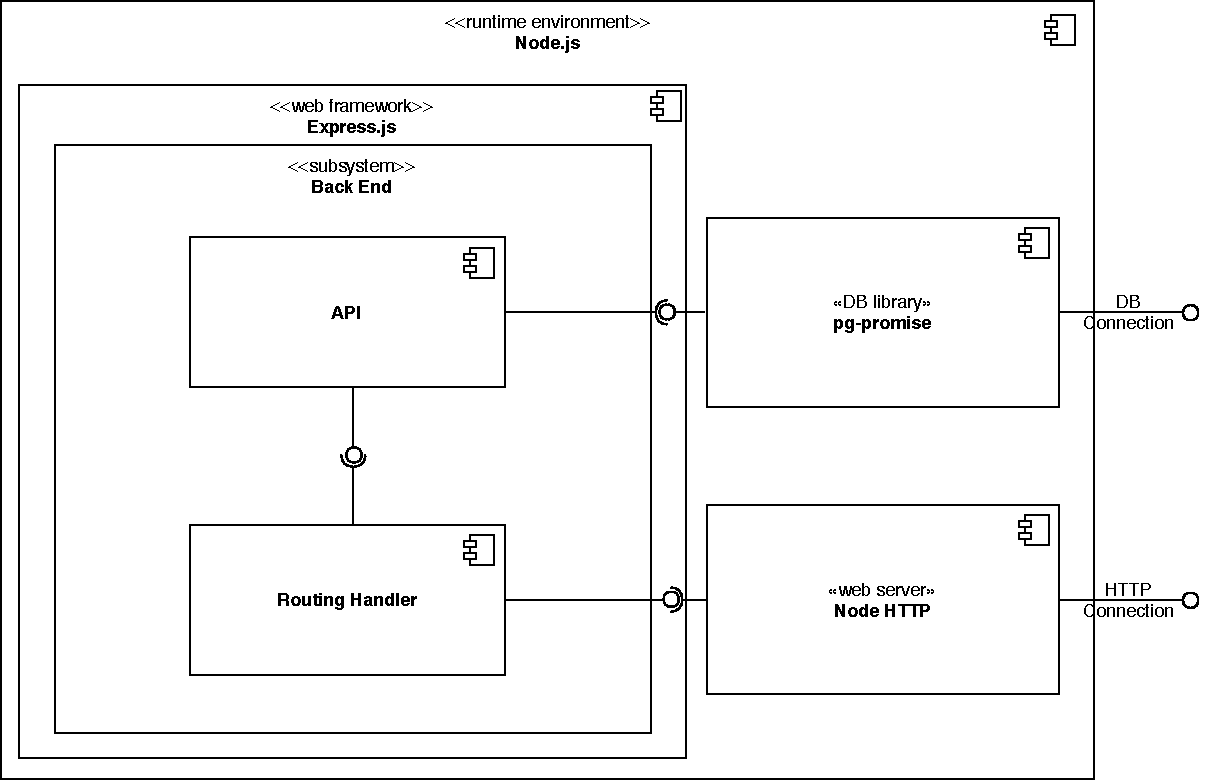
\includegraphics[width=\textwidth,keepaspectratio]{impl_back_end_components.pdf}
	\caption{A component diagram showing the components of the web application's back end.}
	\label{fig:back_end_components}
\end{figure}
The components of the application's back end, its relation to Node.js and Express.js and its top-level external library dependencies are shown in Figure \ref{fig:back_end_components}. Both the back end itself and the external libraries required by it run inside the Node.js runtime environment. 

Two of the back end's components were implemented using the interfaces provided by Express.js: the \textit{Application Programming Interface} (API) and the \textit{Routing Handler}. The API contains the implementations of the functions called by the front end using standard HTTP GET and POST requests. Each of these functions parses parameters contained in a client's request, processes them, creates one or more SQL queries for FREDDY from them, relays the queries to the database using a database driver and produces an HTTP response from the result. The \textit{routing handler} parses the URL of a client's request. If the client requests an API URL, it dispatches the request to the respective API function in order to return dynamic content generated by it. It is also used to determine what static content should be returned as a response to a client's request, such as a web page, a CSS stylesheet or JavaScript code.

The web application's back end delegates communication with the word-embedding enabled database system to \textit{pg-promise}, a database library built on top of \textit{node-postgres}, the Node.js database driver for PostgreSQL. The library was chosen over the lower-level database driver for its features of automatic connection management and pooling, automatic transactions, query formatting and asynchronous operations, of which the API makes use. Communicating over HTTP is also handled by an external Node.js library: \textit{Node HTTP}. It is one of the core modules in Node.js and functions as a web server, listening for client requests and responding to them. The routing handler registers with the web server at the application's initialization to redirect client requests appropriately.

\subsection{API Description}
The web application's API conforms to Representational State Transfer (REST) principles and makes use of HTTP GET and POST requests, as well as JSON-formatted responses, to exchange data between the front end and the back end. Twelve API functions have been implemented. The first seven of them only wrap FREDDY's built-in word embedding operations. The remaining five have been implemented specifically for the web application's use cases. These include a function fetching information about a schema in the database, a function passing a custom query to the database, a function applying user-defined settings to the database, a special k-NN performance test function and a command for the database to pre-load required index tables into the server's RAM. All of the API functions except for the settings function are called by the client via a parameterized HTTP GET request and return a response containing the function's results in a JSON format. See Table \ref{tab:apitable} in Appendix \ref{sec:api-description} for a technical description of the back end's API.

The performance test function uses a list containing one thousand predefined k-NN query terms and their raw results to send a number of k-NN queries for random terms to the database and calculate the average precision and execution time of the operations, comparing to the predefined raw results.

The settings function can be invoked via a POST request carrying a settings object in a custom format (see Table \ref{tab:settings-format} in Appendix \ref{sec:api-description} for the format's description).

\subsection{Example API Call}
\begin{figure}
	\centering
	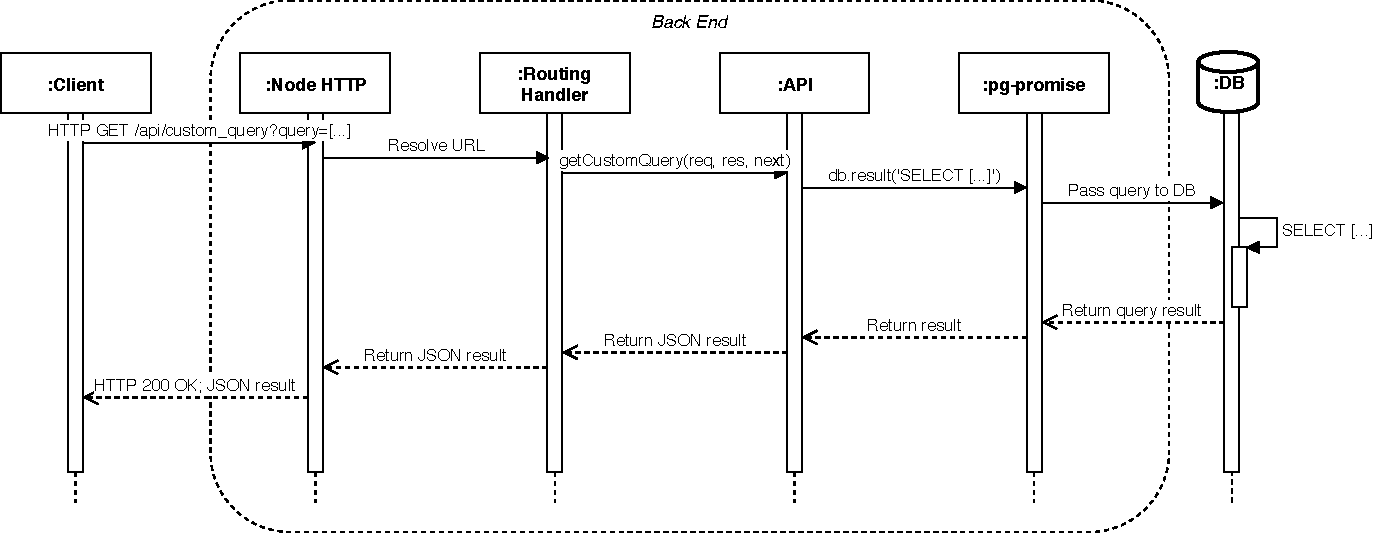
\includegraphics[width=\textwidth, keepaspectratio]{impl_api_seq.pdf}
	\caption{A sequence diagram showing an example interaction with the web application's back end.}
	\label{fig:api_seq}
\end{figure}
Figure \ref{fig:api_seq} shows the interactions between the different back end components, the client and the database when an API function is invoked. A client requests the execution of a user-defined query by sending an HTTP GET request to the listening web server. The Node HTTP instance uses the routing handler to resolve the requested URL, which invokes the respective API function implementation. It builds an SQL query from the client's request and calls a method of pg-promise's API in order to forward the query to the database. The database processes the query and returns the result to the back end, which is converted into a JSON response by the back end's API. The JSON response is then forwarded via the routing handler to the web server, which responds with a 200 OK HTTP message containing the query's results in its body. The JSON data can then be used to present the query's results in the front end's graphical user interface.

\section{Front End}
\subsection{Languages Used}
The web application's front end was implemented in the standard languages used for web development. HTML5 was used for web page markup, CSS3 for describing the content's presentation and JavaScript for the application's front-end logic and DOM manipulation. Furthermore, the web application makes use of several web development frameworks and their respective libraries, as well as external components.

\subsection{Implementation}
\begin{figure}
	\centering
	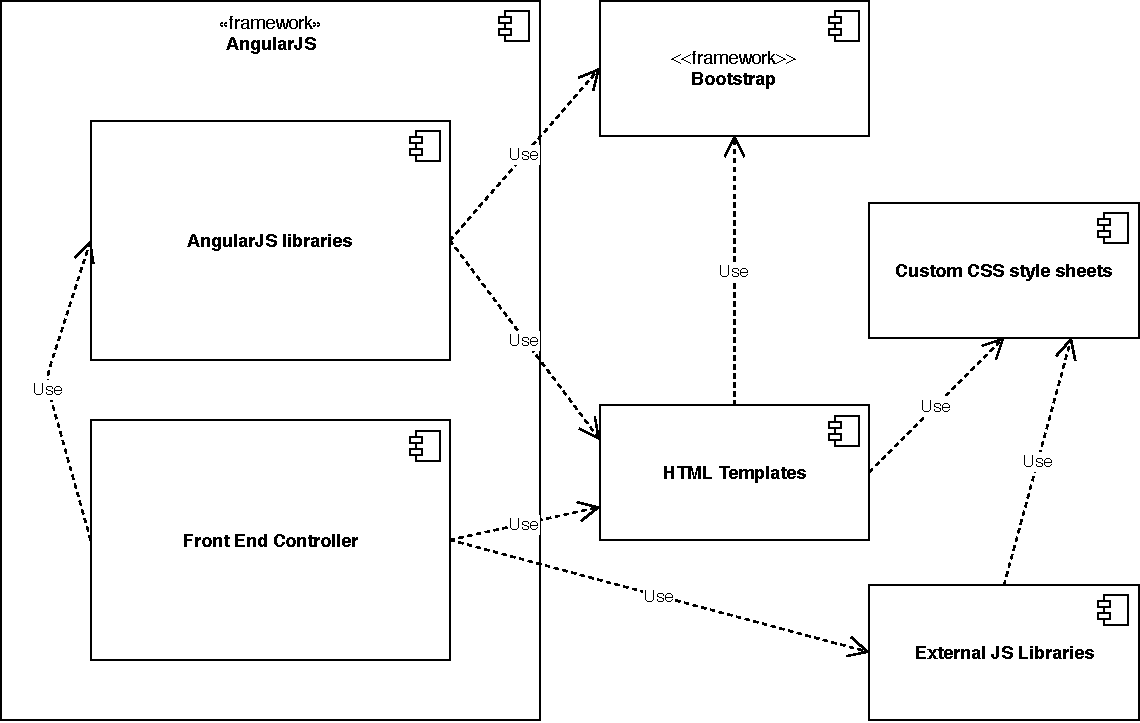
\includegraphics[width=\textwidth, keepaspectratio]{impl_front_end_components.pdf}
	\caption{A component diagram showing the components of the web application's front end.}
	\label{fig:front_end_components}
\end{figure}
Figure \ref{fig:front_end_components} shows an overview of the front end's components and their dependencies. The web application's front end was implemented as a single-page application using the open source web framework \textit{AngularJS}. AngularJS greatly simplifies web application development by presenting a high level of abstraction to the developer. It supports the Model-View-Controller (MVC) paradigm and provides data binding and dependency injection, which is why it was chosen for this project over using pure JavaScript with HTML. AngularJS is a completely client-side framework and runs in the user's browser, thus separating the server side from the client side. Furthermore, it is completely modular and provides many libraries for common tasks, including libraries used for graphical user interface design or HTTP communication. The framework guides the developer through the whole process of building a web application, including designing the user interface and writing the business logic \cite{angularjs-guide}.

AngularJS functions by extending standard HTML by its own directives, attaching specified behavior to HTML elements. Templates written in HTML using AngularJS directives are transformed by the framework into a \textit{view} in the MVC model. The business logic behind views is contained in a \textit{controller}, and a \textit{scope} accessible by both controllers and directives is used to store the data model \cite{angularjs-guide}. In this web application, a controller is used for all client-side logic: sending requests to the back end and processing its responses, presenting data, manipulating the user interface and storing relevant data in the model. Additionally, the controller makes use of several AngularJS libraries to achieve its tasks:

\begin{itemize}
	\item \textit{angular-ui-bootstrap}, \textit{angular-loading-bar} and \textit{angularjs-slider} for AngularJS directives for commonly used UI elements;
	\item \textit{ngTable} for presenting a query's results in a sortable and filterable table;
	\item \textit{ngAnimate} for UI animations;
	\item \textit{ngRoute} for web page routing;
	\item furthermore, the \textit{\$http} AngularJS service is used for communicating with the application's back end.
\end{itemize}

The web application's controller can be split logically roughly into five different parts, some of them also using external JavaScript libraries:

\begin{enumerate}
	\item \textit{query list and query editor} component: fetches a list of predefined queries from the back end, stores them in the model and provides a syntax-highlighted query editor. For the query editor, the JavaScript component \textit{CodeMirror} was used. 
	\item \textit{schema information} component: fetches information about a database schema's structure from the back end and stores it in the model.
	\item \textit{settings} component: controls the presentation of a settings widget and sends the user-specified settings to the back end.
	\item \textit{query results} component: controls the presentation of query results and provides the features of sorting and filtering them.
	\item \textit{performance view} component: initiates new performance tests by sending a request to the back end, controls the performance chart's presentation and adds new data points to it. For the performance chart, the JavaScript graphing library \textit{plotly.js} was used. 
\end{enumerate}

The front end's interface was developed using the open source \textit{Bootstrap} framework. It contains HTML- and CSS-based design templates for typography, forms, buttons, navigation and other interface components. Reasons for choosing Boostrap include its ease of use and its good integration with other web frameworks, including AngularJS. In this project, \textit{angular-ui-bootstrap} was used for native AngularJS directives based on Bootstrap's markup and CSS, providing ready implementations of commonly used user interface elements. Bootstrap also allows the rapid development of responsive, mobile-friendly web applications. It is valued for its high customizability and is compatible with the custom CSS style sheets used to define the web application's appearance.